\documentclass[a4paper]{article} 
\addtolength{\hoffset}{-2.25cm}
\addtolength{\textwidth}{4.5cm}
\addtolength{\voffset}{-3.25cm}
\addtolength{\textheight}{5cm}
\setlength{\parskip}{0pt}
\setlength{\parindent}{0in}

%----------------------------------------------------------------------------------------
%	PACKAGES AND OTHER DOCUMENT CONFIGURATIONS
%----------------------------------------------------------------------------------------

\usepackage{blindtext} % Package to generate dummy text
\usepackage{charter} % Use the Charter font
\usepackage[utf8]{inputenc} % Use UTF-8 encoding
\usepackage{microtype} % Slightly tweak font spacing for aesthetics
\usepackage{amsthm, amsmath, amssymb} % Mathematical typesetting
\usepackage{float} % Improved interface for floating objects
\usepackage[final, colorlinks = true, 
            linkcolor = black, 
            citecolor = black]{hyperref} % For hyperlinks in the PDF
\usepackage{graphicx, multicol} % Enhanced support for graphics
\usepackage{xcolor} % Driver-independent color extensions
\usepackage{marvosym, wasysym} % More symbols
\usepackage{rotating} % Rotation tools
\usepackage{censor} % Facilities for controlling restricted text
\usepackage{listings, style/lstlisting} % Environment for non-formatted code, !uses style file!
\usepackage{pseudocode} % Environment for specifying algorithms in a natural way
\usepackage{style/avm} % Environment for f-structures, !uses style file!
\usepackage{booktabs} % Enhances quality of tables
\usepackage{tikz-qtree} % Easy tree drawing tool
\tikzset{every tree node/.style={align=center,anchor=north},
         level distance=2cm} % Configuration for q-trees
\usepackage{style/btree} % Configuration for b-trees and b+-trees, !uses style file!
\usepackage[backend=biber,style=numeric,
            sorting=nyt]{biblatex} % Complete reimplementation of bibliographic facilities
\addbibresource{ecl.bib}
\usepackage{csquotes} % Context sensitive quotation facilities
\usepackage[yyyymmdd]{datetime} % Uses YEAR-MONTH-DAY format for dates
\renewcommand{\dateseparator}{-} % Sets dateseparator to '-'
\usepackage{fancyhdr} % Headers and footers
\pagestyle{fancy} % All pages have headers and footers
\fancyhead{}\renewcommand{\headrulewidth}{0pt} % Blank out the default header
\fancyfoot[L]{} % Custom footer text
\fancyfoot[C]{} % Custom footer text
\fancyfoot[R]{\thepage} % Custom footer text
\newcommand{\note}[1]{\marginpar{\scriptsize \textcolor{red}{#1}}} % Enables comments in red on margin

%----------------------------------------------------------------------------------------

\begin{document}

%-------------------------------
%	TITLE SECTION
%-------------------------------

\fancyhead[C]{}
\hrule \medskip % Upper rule
\begin{minipage}{0.295\textwidth} 
\raggedright
\footnotesize
Azure Hutchings \hfill\\   
n9748601 \hfill\\
\end{minipage}
\begin{minipage}{0.4\textwidth} 
\centering 
\large 
Assignment 1 Report\\ 
\normalsize 
CAB402 Programming Paradigms\\ 
\end{minipage}
\begin{minipage}{0.295\textwidth} 
\raggedleft
\today\hfill\\
\end{minipage}
\medskip\hrule 
\bigskip

%-------------------------------
%	CONTENTS
%-------------------------------
\section*{Discussion and Comparison of Pure Functional (F\#) and Object-Oriented Imperative (C\#)}

\subsection*{Efficiency}
To accurately compare the runtime for both the C\# genetics algorithm and the F\# genetics algorithm a comparison was performed. This was done by editing the TSP controller so that the modified code keeps track of the best score so far, and how many generations that has remained the best score. After a stipulated time (500 generations), if no improvement is observed, it sends a diagnostic message to the immediate window and halts the run. This runtime was then recorded in the table below.
\begin{table}[h!]
\centering
 \begin{tabular}{||c c ||} 
 \hline
 F\# & C\# \\ [0.5ex] 
 \hline\hline
 30s & 25s  \\ 
 \hline
 32s & 28s \\
 \hline
 32s & 27s \\
 \hline
 32s & 27s \\
 \hline
 34s & 31s \\
 \hline
 33s & 31s\\[0.5ex]
 \hline
\end{tabular}
\caption{Time taken for the solution to converge for randomised Travelling Salesperson Problem.} \label{tab:efficency}
\end{table}
\\\\
As seen in Table \ref{tab:efficency}, the runtime performance took longer in the C\# program than the F\# for the Travelling Salesperson Problem. 

\subsection*{Effectiveness}
For readability, the F\# was definitely easier to read than the C\# code. The pipes in F\#, as seen in Figure \ref{fig:FSharpSnippet}, allows the code to be written to pass parameters from left to right. This allows the code to be easier to read compared to languages, such as, C\#.

\begin{figure}[H]
	\center
	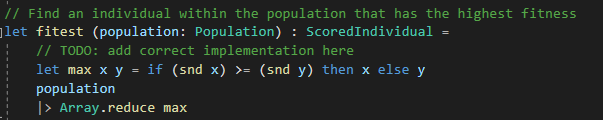
\includegraphics[width=0.9\linewidth]{images/FSharpSnippet.png}
	\caption{F\# Code.}
	\label{fig:FSharpSnippet}
\end{figure}

\begin{figure}[H]
	\center
	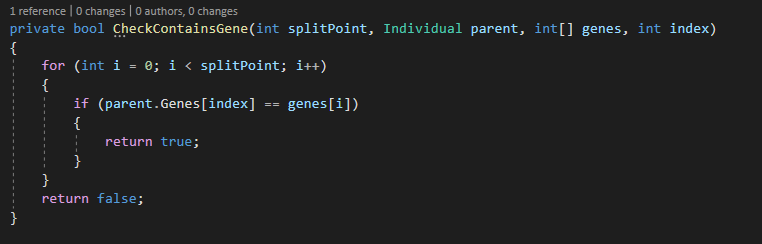
\includegraphics[width=0.9\linewidth]{images/CSharpSnippet.png}
	\caption{C\# Code.}
	\label{fig:CSharpSnippet}
\end{figure}

\begin{figure}[H]
	\center
	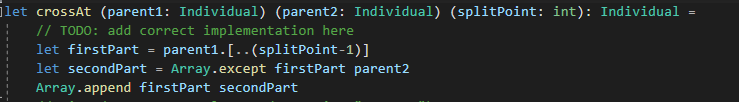
\includegraphics[width=0.9\linewidth]{images/FSharpSnippet2.png}
	\caption{F\# Code.}
	\label{fig:FSharpSnippet2}
\end{figure}
In Figure \ref{fig:CSharpSnippet} and Figure \ref{fig:FSharpSnippet2}, code with similar functions are executed. The \textit{secondPart} in the F\# code performs the same function as the \textit{CheckContainsGene} in the C\# code. Both the \textit{secondPart} and the \textit{CheckContainsGene} are creating/adding to an existing array that does not contain certain elements found in another parent. 
\\\\
In terms of debugging both programs, it was found to be much easier to debug using F\# as 
\\\\
It is evident that the F\# code requires fewer lines than the C\# code and is much easier to read and follow without the use of extensive comments. Pure functional approach is much more concise, easier to read, and produces more efficient code than a object-oriented imperative approach.  
\\\\
In terms of programming using both a pure functional approach and object-oriented approach, it was found that object-oriented took less time to implement than the pure functional approach. This however, could be due to lack of prior understanding of programming if F\# and thus, took longer to comprehend how to effectively program in that language.
\\\\
discussing your experience and comparing the two approaches (F\# pure functional and C\# object-oriented imperative). Your comparison should include a discussion on the efficiency and effectiveness of the two approaches. You should discuss which was easier to program, which code is easier to read, understand and maintain, which is more concise, and which produces more efficient code. Provide measures were applicable to support your claims.

\end{document}
